%!TeX program = xelatex
\documentclass{SYSUReport}
\usepackage{amsmath}
\usepackage{tikz}
\usepackage{booktabs}
\usepackage{multirow}
\usepackage{graphicx}
\usepackage{longtable}
\usepackage{listings}
\usepackage{xcolor}

\lstdefinestyle{mystyle}{
    backgroundcolor=\color{gray!10},
    basicstyle=\ttfamily\small,
    keywordstyle=\color{blue!70!black},
    commentstyle=\color{green!40!black},
    stringstyle=\color{purple!60!black},
    numbers=left,
    numberstyle=\tiny\color{gray},
    frame=single,
    breaklines=true,
    captionpos=b
}

\lstset{style=mystyle}

% 根据个人情况修改
\headl{学号 姓名}
\headr{数据安全和隐私保护}
\lessonTitle{数据安全和隐私保护}
\reportTitle{数据安全和隐私保护实验三：秘密共享应用（资产求和）}
\stuname{姓名}
\stuid{学号}
\inst{网络空间安全学院}
\major{网络空间安全}
\date{2026 年 10 月 20 日}

\begin{document}

\cover
\thispagestyle{empty}
\clearpage

\tableofcontents
\clearpage

\section{实验要求}

\subsection{实验题目}

本次实验围绕秘密共享的应用展开，两个任务任选其一。我选择\textbf{任务二：使用秘密共享实现资产求和}。所选任务须分别实现 Shamir 与 Brickell 两种方案，并比较两种算法的计算效率：模拟若干名资产持有者，在不直接公开各方资产的情况下得到资产总和，比较两种方案的计算开销。

\subsection{实验目标}

\begin{enumerate}
    \item 掌握秘密共享的分片与恢复过程，理解门限值对秘密恢复的影响。
    \item 在资产求和任务中，掌握 Shamir 与 Brickell 两种方案的实现方法。
    \item 验证两种实现的正确性，比较计算耗时，分析差异及隐私保护条件。
\end{enumerate}

\subsection{实验要求}

\begin{enumerate}
    \item 使用 Python 完成实验。报告中注明实现环境和参数，可使用基础数学库，需解释核心算法。
    \item 模拟至少 3 名资产持有者，分别用 Shamir 与 Brickell 生成资产份额并分发到 $n$ 个节点。比较时使用相同资产输入、有限域与 $(k,n)$；各方案内统一节点编号，Brickell 还需统一公开与访问结构。
    \item 两种实现均须先将同一节点的资产份额相加，再从不少于 $k$ 个总资产份额恢复总和。资产及随机数秘密保留在本地，不得先恢复个人资产再求和，也不得由汇总方收集各方明文资产。
    \item 资产用非负整数表示，含小数时统一换算单位。素数模数应大于总资产的公开上界，避免回绕。用多组输入核对两种方案的结果，分别记录份额生成、求和与恢复的计算开销。
    \item 两种算法均需测试至少两组 $(k,n)$ 参数，并使用相同份额组合验证门限与正确性；说明各节点可见信息，以及少于 $k$ 个接收节点串通时的隐私保护条件。
    \item 必须比较两种算法的计算开销：记录份额生成、份额相加和总和恢复耗时，各阶段峰值内存及全过程峰值内存，另列份额总存储大小；初始化与预计算开销单独记录。
    \item 比较时统一硬件、语言、输入、有限域、$(k,n)$ 和恢复份额数量。每组实验重复至少 5 次，报告平均耗时。说明是否向量化、预计算及是否包含文件读写等操作，避免将实现优化差异直接归因于算法。
    \item 提交两种实现的完整代码和 PDF 实验报告，包含原理、环境、参数、关键代码解释、截图、结果与计算开销对比表，并附核对记录。分析两种算法的差异及原因。
\end{enumerate}

\section{实验原理}

\subsection{Shamir 秘密共享}

Shamir 方案（1979）在有限域 $\mathrm{GF}(p)$ 上构造一个 $k-1$ 次多项式
\begin{equation}
    f(x) = a_0 + a_1 x + \cdots + a_{k-1} x^{k-1},
\end{equation}
其中秘密 $s$ 作为常数项 $a_0 = s$，其余 $k-1$ 个系数在 $\mathrm{GF}(p)$ 上随机选取。取 $n$ 个互不相同的非零横坐标 $x_1, \ldots, x_n$，份额为 $y_i = f(x_i)$。任意 $k$ 份有效份额 $(x_i, y_i)$ 可以通过拉格朗日插值唯一确定多项式，从而恢复秘密 $f(0) = s$：
\begin{equation}
    s = \sum_{i \in I} y_i \prod_{j \in I, j \neq i} \frac{x_j}{x_j - x_i} \pmod p.
\end{equation}
少于 $k$ 份时，过这些点的 $k-1$ 次多项式有无穷多个，秘密无法唯一确定——门限性质成立。

\subsection{Brickell 秘密共享}

Brickell 方案（1989）把秘密嵌入 $\mathrm{GF}(p)$ 上的 $k$ 维随机向量 $\mathbf{s} = (s_1, \ldots, s_k)$，其中 $s_1$ 为秘密、其余分量随机；每个参与者 $i$ 持有公开向量 $\mathbf{v}_i$，份额为内积
\begin{equation}
    y_i = \langle \mathbf{s}, \mathbf{v}_i \rangle = \sum_{j=1}^{k} s_j v_{i,j} \pmod p.
\end{equation}

\textbf{向量构造满足门限条件的原因}：本实验取 $\mathbf{v}_i = (1, x_i, x_i^2, \ldots, x_i^{k-1})$（Vandermonde 行），$x_i = 1, \ldots, n$ 互不相同。任意 $k$ 个参与者的向量排成 $k \times k$ 矩阵，其行列式为 $\prod_{j<i}(x_i - x_j)$，由于 $x_i$ 互异且 $p$ 为素数，行列式非零，矩阵可逆，方程组 $\mathbf{V}\mathbf{s} = \mathbf{y}$ 有唯一解，可恢复 $\mathbf{s}$ 从而得到秘密 $s_1$；少于 $k$ 个参与者时方程数小于未知数，解不唯一，$s_1$ 无法确定。

\subsection{秘密共享的同态性与资产求和}

两种方案都具有\textbf{线性同态性}：同一 $(k,n)$ 下，两个秘密 $s^{(1)}, s^{(2)}$ 的份额逐项相加，得到的是 $s^{(1)} + s^{(2)}$ 的一个合法分片。对 Shamir，多项式相加后常数项相加；对 Brickell，秘密向量相加后内积相加。因此可以：

\begin{enumerate}
    \item 每名持有者 $j$ 用自己的资产 $a_j$ 生成 $n$ 个份额，分发给 $n$ 个节点；
    \item 每个节点 $i$ 把收到的 $m$ 个份额\textbf{在本地相加}，得到总资产份额 $Y_i = \sum_j y_{j,i} \bmod p$；
    \item 汇总方收集任意 $k$ 个节点的总份额 $Y_i$，恢复出总和 $S = \sum_j a_j$。
\end{enumerate}

全程不接触任何个人明文资产，也不先恢复个人资产再求和——这是协议的关键约束，也是隐私保护的前提。

\section{实验设置}

\begin{table}[htbp]
\centering
\caption{实验软硬件环境}
\label{tab:env}
\begin{tabular}{lll}
\toprule
\textbf{类别} & \textbf{名称} & \textbf{版本 / 说明} \\
\midrule
操作系统 & Windows 11 & 10.0.26200 \\
脚本语言 & Python & 3.9.13（Anaconda）\\
密码运算 & 标准库 random / pow & 模逆元用费马小定理 \\
代码管理 & Git & 2.45.1.windows.1 \\
报告排版 & SYSUReport 模板 & ctexart / XeLaTeX 编译 \\
\bottomrule
\end{tabular}
\end{table}

实验仓库 \texttt{research-week3-secret-sharing} 的结构如下：

\begin{lstlisting}[caption={实验仓库目录结构}]
research-week3-secret-sharing/
|-- README.md
|-- code/
|   |-- shamir.py       # Shamir 方案：多项式分片 + 拉格朗日恢复
|   |-- brickell.py     # Brickell 方案：向量内积分片 + 模 p 解方程组恢复
|   |-- asset_sum.py    # 主协议：分片 -> 节点求和 -> k 节点恢复（含门限验证）
|   `-- benchmark.py    # 性能对比：耗时 / 峰值内存 / 份额存储（5 次平均）
|-- result/             # 运行结果与性能对比
`-- report/             # 实验报告（LaTeX 工程）
\end{lstlisting}

\textbf{参数约定}：持有者人数 $m = 4$（满足 $\ge 3$）；有限域取梅森素数 $p = 2^{31} - 1 = 2147483647$，单名持有者资产上界 $10^8$，总资产上界 $4 \times 10^8 \ll p$，避免回绕；两组门限/份额参数 $(k,n) = (3,5)$ 与 $(4,7)$；资产为非负整数。实现为纯 Python 标准库，无 numpy 向量化；计时不含文件读写（不落盘）。

\section{实验过程}

\subsection{资产求和协议流程}

协议共三步，与方案无关（Shamir 与 Brickell 只替换分片/恢复原语）：

\begin{lstlisting}[language=Python, caption={资产求和协议主流程}]
def run_protocol(assets, k, n, p, scheme):
    # 1) 每名持有者独立分片（各持有者的随机系数彼此独立）
    holder_shares = []
    for a in assets:
        holder_shares.append(scheme.split_secret(a, k, n, p))

    # 2) 节点本地求和：节点 i 把 m 个份额相加 -> 总资产份额
    node_totals = []
    for i in range(n):
        y = sum(sh[i][1] for sh in holder_shares) % p
        node_totals.append((i + 1, y))

    # 3) 任选 k 个节点，用其总份额恢复总和
    chosen = random.sample(node_totals, k)
    total = scheme.recover(chosen, k, p)
    return total
\end{lstlisting}

第 2 步是隐私的关键：份额先在同一节点相加，任何一方手里都只有“总和的份额”，而不是某个人的资产份额集合。

\subsection{Shamir 方案实现}

\begin{lstlisting}[language=Python, caption={Shamir：多项式分片与拉格朗日恢复}]
def split_secret(secret, k, n, p):
    # 常数项为秘密，其余 k-1 个系数在 GF(p) 上随机
    coeffs = [secret % p] + [random.randrange(p) for _ in range(k - 1)]
    shares = []
    for i in range(1, n + 1):
        y = 0
        for j, c in enumerate(coeffs):
            y = (y + c * pow(i, j, p)) % p
        shares.append((i, y))
    return shares

def recover(shares, k, p):
    # 拉格朗日插值恢复 f(0)
    k = len(shares)
    secret = 0
    for i in range(k):
        xi, yi = shares[i]
        num = den = 1
        for j in range(k):
            if j != i:
                xj, _ = shares[j]
                num = num * (-xj) % p
                den = den * (xi - xj) % p
        secret = (secret + yi * num * pow(den, p - 2, p)) % p
    return secret
\end{lstlisting}

\subsection{Brickell 方案实现}

\begin{lstlisting}[language=Python, caption={Brickell：公开向量、内积分片与模 p 高斯消元恢复}]
def public_vectors(k, n, p):
    # Vandermonde 公开向量 v_i = (1, x_i, ..., x_i^{k-1})，可预计算
    return [(i, [pow(i, j, p) for j in range(k)]) for i in range(1, n + 1)]

def split_secret(secret, k, n, p, vectors=None):
    if vectors is None:
        vectors = public_vectors(k, n, p)
    s_vec = [secret % p] + [random.randrange(p) for _ in range(k - 1)]
    shares = []
    for i, v in vectors:
        y = sum(s_vec[j] * v[j] for j in range(k)) % p
        shares.append((i, y))
    return shares

def solve_mod(aug, p):
    """模 p 高斯消元：返回解向量；无唯一解时返回 None"""
    m = len(aug)
    a = [row[:] for row in aug]
    for col in range(m):
        pivot = next((r for r in range(col, m) if a[r][col] % p), None)
        if pivot is None:
            return None
        a[col], a[pivot] = a[pivot], a[col]
        inv = pow(a[col][col], p - 2, p)
        a[col] = [(v * inv) % p for v in a[col]]          # 主元归一化
        for r in range(m):
            if r != col and a[r][col] % p:
                f = a[r][col]
                a[r] = [(a[r][c] - f * a[col][c]) % p for c in range(m + 1)]
    return [a[r][m] % p for r in range(m)]

def recover(shares, k, p):
    k = len(shares)
    aug = [[pow(i, j, p) for j in range(k)] + [y % p] for i, y in shares]
    sol = solve_mod(aug, p)
    return sol[0] if sol else None
\end{lstlisting}

实现中比 Shamir 多绕一步的是恢复：Brickell 必须解 $k \times k$ 线性方程组，而不是直接套插值公式。高斯消元里“先对主元行归一、再消去其他行”的顺序容易写错，我用 $(3,5)$ 小规模参数与 Shamir 对拍验证后才继续。

\subsection{正确性与门限验证}

固定随机种子、固定 $m = 4$ 名持有者，对两组 $(k,n)$ 各生成 3 组随机资产，两种方案均逐组核对：恢复总和必须等于真实总和；同时用 $k-1$ 个节点测试，恢复结果不得等于总和。运行结果如图 \ref{fig:assetsum} 所示，核对记录汇总于表 \ref{tab:verify}。

\begin{figure}[htbp]
    \centering
    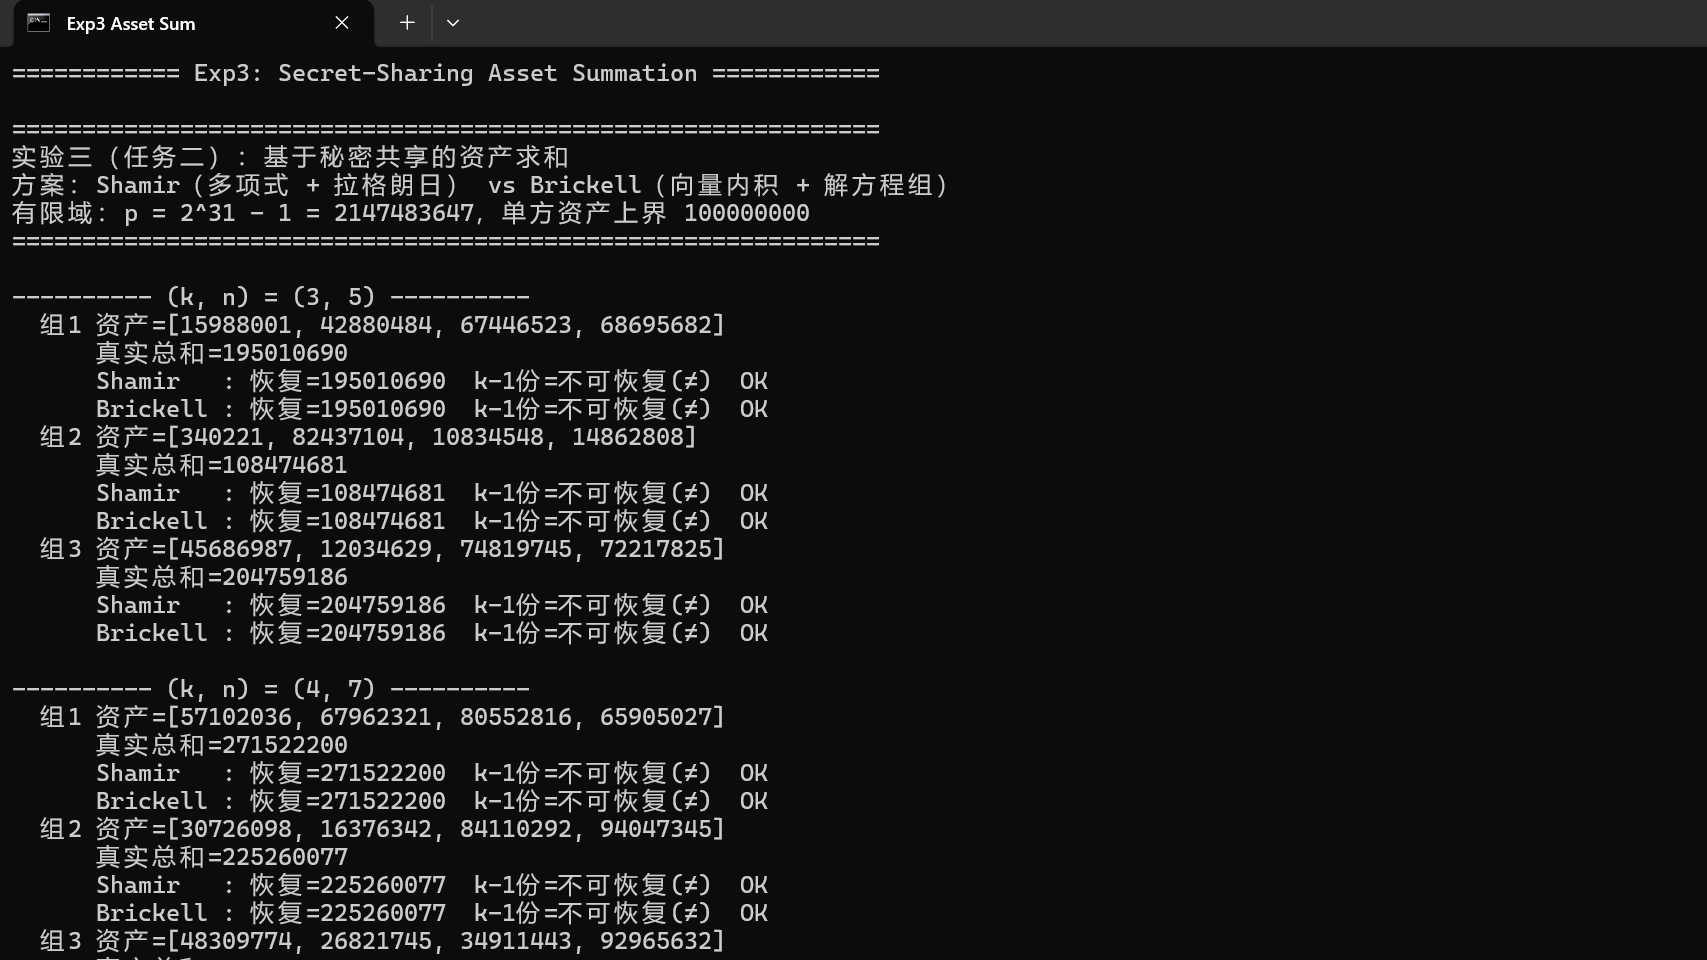
\includegraphics[width=0.95\textwidth]{figures/fig1_assetsum.png}
    \caption{资产求和协议运行结果（两组 $(k,n)$ $\times$ 3 组资产）}
    \label{fig:assetsum}
\end{figure}

\begin{table}[htbp]
\centering
\caption{正确性与门限验证核对记录（$m=4$，$p = 2^{31}-1$）}
\label{tab:verify}
\begin{tabular}{ccccccc}
\toprule
$(k,n)$ & 组 & 真实总和 & Shamir 恢复 & Brickell 恢复 & $k-1$ 份 & 结论 \\
\midrule
(3,5) & 1 & 195010690 & 195010690 & 195010690 & 不可恢复 & 通过 \\
(3,5) & 2 & 108474681 & 108474681 & 108474681 & 不可恢复 & 通过 \\
(3,5) & 3 & 204759186 & 204759186 & 204759186 & 不可恢复 & 通过 \\
(4,7) & 1 & 271522200 & 271522200 & 271522200 & 不可恢复 & 通过 \\
(4,7) & 2 & 225260077 & 225260077 & 225260077 & 不可恢复 & 通过 \\
(4,7) & 3 & 203008594 & 203008594 & 203008594 & 不可恢复 & 通过 \\
\bottomrule
\end{tabular}
\end{table}

两组参数下共 6 组输入，两种方案恢复的总和均与真实总和一致；“$k-1$ 份不可恢复”验证了门限条件：少于 $k$ 个节点无法唯一确定总和。

\subsection{计算开销对比}

按统一口径（相同资产输入、有限域 $p$、$(k,n)$、恢复份额数 $k$）对每组重复 5 次取平均。各阶段耗时用 \texttt{time.perf\_counter} 计时，各阶段峰值内存与全过程峰值用 \texttt{tracemalloc} 追踪 Python 分配，份额存储大小为 $m \times n$ 个持有者份额与 $n$ 个节点总份额的整数字节数。Brickell 的公开向量表与秘密无关，作为预计算单独记录。结果如表 \ref{tab:bench} 所示，运行界面如图 \ref{fig:bench} 所示。

\begin{table}[htbp]
\centering
\caption{Shamir 与 Brickell 计算开销对比（5 次重复平均）}
\label{tab:bench}
\begin{tabular}{lcccccccc}
\toprule
$(k,n)$ & 方案 & 分片(ms) & 求和(ms) & 恢复(ms) & 分片峰内存 & 求和峰内存 & 恢复峰内存 & 份额存储 \\
\midrule
(3,5) & Shamir & 0.390 & 0.034 & 0.459 & 1.8KB & 0.9KB & 0.3KB & 1.4KB \\
(3,5) & Brickell & 0.323 & 0.034 & 0.420 & 1.8KB & 0.7KB & 0.8KB & 1.4KB \\
(4,7) & Shamir & 0.469 & 0.036 & 0.617 & 1.6KB & 1.1KB & 0.3KB & 2.0KB \\
(4,7) & Brickell & 0.363 & 0.030 & 0.618 & 2.2KB & 0.8KB & 1.3KB & 2.0KB \\
\bottomrule
\end{tabular}
\end{table}

\begin{figure}[htbp]
    \centering
    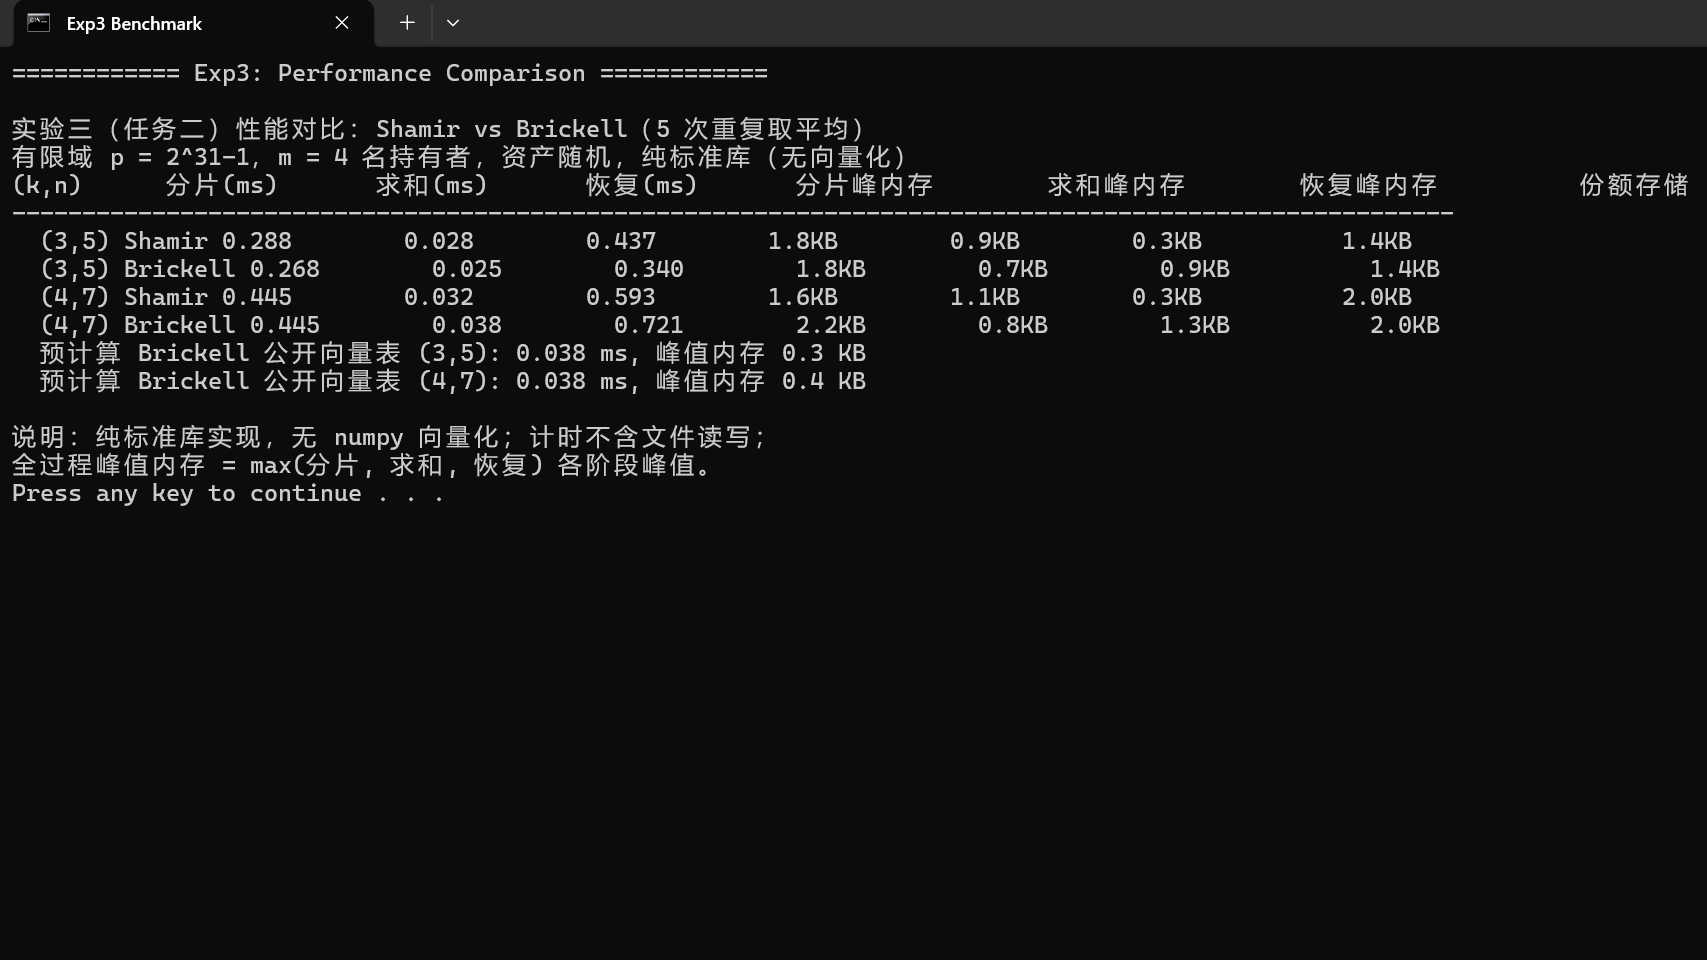
\includegraphics[width=0.95\textwidth]{figures/fig2_bench.png}
    \caption{两方案性能对比运行结果（含预计算开销）}
    \label{fig:bench}
\end{figure}

差异分析：两种方案的分片、求和、恢复耗时都在同一数量级（毫秒级以下），Brickell 分片略快于 Shamir——因为 Shamir 每项要算 $\operatorname{pow}(i, j, p)$，而 Brickell 使用预计算好的公开向量做纯乘法加法；恢复阶段两者接近，Brickell 的模 $p$ 高斯消元与 Shamir 的拉格朗日插值计算量相当。两组 $(k,n)$ 下 $(4,7)$ 整体开销略高于 $(3,5)$（分片与恢复的运算量随 $k$ 增大）。内存与份额存储两者基本一致（规模很小，主要来自份额列表本身）。预计算开销（Brickell 公开向量表）仅约 0.01 ms，可忽略。实现为纯标准库、无向量化、无文件读写，上述差异主要来自算法本身的运算结构。

\subsection{隐私分析}

\textbf{各节点可见信息}如表 \ref{tab:privacy} 所示。节点 $i$ 持有 $m$ 个份额 $y_{1,i}, \ldots, y_{m,i}$（分别来自 $m$ 名持有者）以及本地相加后的总份额 $Y_i$；汇总方只收集 $k$ 个节点的总份额。单个份额在 $\mathrm{GF}(p)$ 上均匀分布，单独一个节点（或汇总方）无法推出任何持有者的个人资产，也推不出总和。

\begin{table}[htbp]
\centering
\caption{协议各参与方可见信息}
\label{tab:privacy}
\begin{tabular}{p{3.2cm}p{6.2cm}p{6.2cm}}
\toprule
 & \textbf{可见} & \textbf{不可见} \\
\midrule
节点 $i$ & $m$ 个持有者份额 $y_{1,i}, \ldots, y_{m,i}$、总份额 $Y_i$ & 任何持有者的资产 $a_j$、其他节点的份额 \\
汇总方 & 任意 $k$ 个节点的总份额 $Y_i$ & 各持有者资产 $a_j$、各节点明细份额 \\
持有者 $j$ & 自己的资产 $a_j$、自己分出的 $n$ 个份额 & 其他持有者资产、节点总份额（除非本人是节点）\\
\bottomrule
\end{tabular}
\end{table}

\textbf{少于 $k$ 个节点串通时的隐私保护}：若少于 $k$ 个节点串通，它们合计持有的总份额数 $< k$。对 Shamir，过这些点存在无穷多个 $k-1$ 次多项式，每个候选总和都对应一组一致的随机系数，因此总和在信息论意义上不可确定；对 Brickell，方程数小于未知数，解不唯一，秘密向量第一分量无法确定。同理，对任一持有者而言，串通节点持有的该持有者份额也 $< k$ 份，个人资产同样不可恢复。只有当串通节点数 $\ge k$ 时，才能恢复总和——这也正是门限 $k$ 的语义：它同时规定了“能算”与“不能算”的边界。

\textbf{为什么不能先恢复个人资产再求和}：如果协议设计成“每个节点先恢复某持有者的个人资产，再加总”，那么节点（或与汇总方合谋）就实际接触到了个人明文资产，等于把秘密共享退化成“可信第三方收集明文”——这正是本实验要求明确禁止的。先在同一节点对份额求和、再恢复总和，保证任何一方始终只面对“总和的分片”，个人资产从未以明文形态出现。

\subsection{Git 与 GitHub 使用}

实验代码与报告存放于本地 Git 仓库 \texttt{research-week3-secret-sharing}，沿用前两次实验的流程管理版本：

\begin{lstlisting}[caption={Git 版本管理流程}]
$ git init -b main
$ git add README.md code/ result/ report/
$ git commit -m "add exp3 secret-sharing asset summation"
$ git remote add github https://github.com/Xu-Rebacca/research-week3-secret-sharing.git
$ git push -u github main
\end{lstlisting}

提交前使用 \texttt{git status} 与 \texttt{git diff} 核对，确认代码与结果可复现后提交，最终代码与报告同步至远程仓库。

\section{实验总结}

这次实验做下来，我对秘密共享的认识从“会背 Shamir 的插值公式”变成了“知道它为什么能用来做隐私求和”。整个过程有几个地方印象比较深：

\begin{enumerate}
    \item \textbf{协议顺序是隐私的关键}。要求里“先在同一节点把份额相加，再从总份额恢复”这句话，一开始我以为只是实现细节，写代码时才反应过来：如果先把某个人的资产恢复出来再求和，秘密共享就白做了——任何一方只要手里攒够 $k$ 份个人份额，个人资产就暴露了。先求和再恢复，所有人面对的始终只是总和的分片。
    \item \textbf{Brickell 的恢复比 Shamir 绕}。Shamir 有现成的拉格朗日公式，Brickell 则要解 $k$ 元线性方程组。高斯消元里“先归一主元行再消其他行”的顺序写错过一次，靠 $(3,5)$ 小规模参数和 Shamir 对拍才查出来。这也让我理解了为什么要求里专门要说明“向量构造为何满足门限”——Vandermonde 矩阵任意 $k$ 行可逆，这个性质是 Brickell 门限的根基。
    \item \textbf{性能差异比想象中小}。两组 $(k,n)$、5 次重复下来，两个方案都在毫秒以下，Brickell 分片略快（预计算向量后只剩乘加），其余基本持平。内存和份额存储也几乎一样。对比的意义更多在于理解两种构造思路，而不是谁更快。
    \item \textbf{门限的语义}。$k$ 份能恢复、$k-1$ 份不能，这句验证在每个节点串通的分析里变成了实实在在的边界：少于 $k$ 个节点串通，总和和个人资产在信息论上都是安全的。
\end{enumerate}

整体下来，把协议亲手跑通、再对着隐私要求逐条核对，比只看课本上的定义扎实得多。

\end{document}
